% Dokumentenart und Schriftgröße
\documentclass[
    12pt,
    a4paper
]{article}

% Verfügbarmachen externer Funktionalitäten
\usepackage[
    left=4cm,
    right=1.5cm,
    top=3cm,
    bottom=2cm
]{geometry}
\usepackage[
    toc,
    style=alttree,
    acronym,
    nopostdot,
    nonumberlist
]{glossaries}
\usepackage[ngerman]{babel}
\usepackage[export]{adjustbox}
\usepackage[titles]{tocloft}
\usepackage[
    backend=biber,
    style=numeric
]{biblatex}
\usepackage[T1]{fontenc}
\usepackage{verbatim}
\usepackage{minted}
\usepackage{hyperref}
\usepackage{setspace}
\usepackage{graphicx}
\usepackage{ragged2e}
\usepackage{fontspec}
\usepackage{fancyhdr}
\usepackage{svg}
\usepackage{tocbibind}
\usepackage{float}

% Datei, welche die Einträge für das Literaturverzeichnis enthält
\addbibresource{bibliography.bib}

% Pfad zu Bildern setzen
\graphicspath{{img/}}

% Abkürzungsverzeichnis
\makeglossaries

% Liste verwendeter Abkürzungen
\newacronym{hcc}{HCC}{Hessisches Competence Center}

% Einrückungen im Abbildungsverzeichnis verhindern
\renewcommand\cftfigindent{0pt}

% Seitenzahl in oberer rechter Ecke einblenden
\pagestyle{fancy}
\fancyhf{}
\fancyhead[R]{\thepage}
\renewcommand{\headrulewidth}{0pt}

% Schriftart des Dokuments
\setmainfont{Arial}

% Design des Syntax-Highlightings
\usemintedstyle{staroffice}

% Inhaltsverzeichnis ohne Punkte zwischen Überschrift und Seitenzahl
\renewcommand{\cftdot}{}

% PDF-Einstellungen
\hypersetup{
    colorlinks=true,
    citecolor=black,
    linkcolor=black,
    urlcolor=blue,
    pdftitle={Projektstudium im SS 23}
}

% Zeilenabstand
\setstretch{1.5}

\begin{document}

% Seitennummerierung deaktivieren
\pagenumbering{gobble}

% Logo-Bereich
\noindent
\begin{minipage}[t]{\textwidth}
    \raisebox{-0.28cm}{\includesvg[height=1.7cm]{logo_thm}}
    \hfill
    \includesvg[height=1.7cm]{logo_sp}
\end{minipage}\\[.5cm]

\begin{Center}
    \textbf{Projektstudium im SS 23\\[1cm]}
\end{Center}

\noindent
Thema:\\
\textbf{Projektthema\\[1.5cm]}

% Angaben zum Studenten und der Behörde
\begin{FlushLeft}
    \begin{tabular}{@{} l @{\hspace{2.5cm}} p{.5\linewidth} @{}}
        Vorgelegt von:     & Max Mustermann                                                        \\
                           & Straße 8                                                              \\
                           & 12345 Musterstadt                                                     \\
        Matrikelnummer:    & 123456789                                                             \\[1.5cm]
        Eingereicht bei                                                                            \\
        Hochschulbetreuer: & Prof. Dr. Hans Meier                                                  \\
        Fachbetreuer:      & Herr Frank Müller                                                     \\[1.5cm]
        Behörde:           & Hessisches Competence Center für Neue Verwaltungssteuerung, Wiesbaden \\
        Eingereicht am:    & 15.02.2022
    \end{tabular}
\end{FlushLeft}

\clearpage

% Kapitel ohne Nummerierung und Aufführung im Inhaltsverzeichnis
\section*{Sperrvermerk}
Der vorliegende Projektbericht beinhaltet interne vertrauliche Informationen des Hessischen Competence Centers.\\
Die Weitergabe des Inhaltes der Arbeit und eventuell beiliegender Zeichnungen und Daten im Gesamten oder in Teilen ist grundsätzlich untersagt.
Es dürfen keinerlei Kopien oder Abschriften - auch in digitaler Form - gefertigt werden.
Ausnahmen bedürfen der schriftlichen Genehmigung des Hessischen Competence Centers.

\clearpage

% Seitennummerierung mit großen römischen Zahlen
\pagenumbering{Roman}

% Inhaltsverzeichnis
\tableofcontents

\clearpage

% Angaben zum Abkürzungsverzeichnis
\glsfindwidesttoplevelname
\printglossary[
    type=\acronymtype,
    title=Abkürzungsverzeichnis,
    toctitle=Abkürzungsverzeichnis
]

\clearpage

% Abbildungsverzeichnis
\listoffigures

\clearpage

% Seitennummerierung mit arabischen Zahlen
\pagenumbering{arabic}

\section{Einleitung}
\subsection{Hessisches Competence Center}
Das 2001 gegründete Hessische Competence Center für Neue Verwaltungssteuerung in Wiesbaden (\acrshort{hcc}) ist ein SAP-,
Finanz- und Beschaffungsdienstleister,
der die rund 800 hessischen Landesdienststellen unterstützt \cite{hcc-ueber-uns}.

\begin{figure}[H]
    \centering
    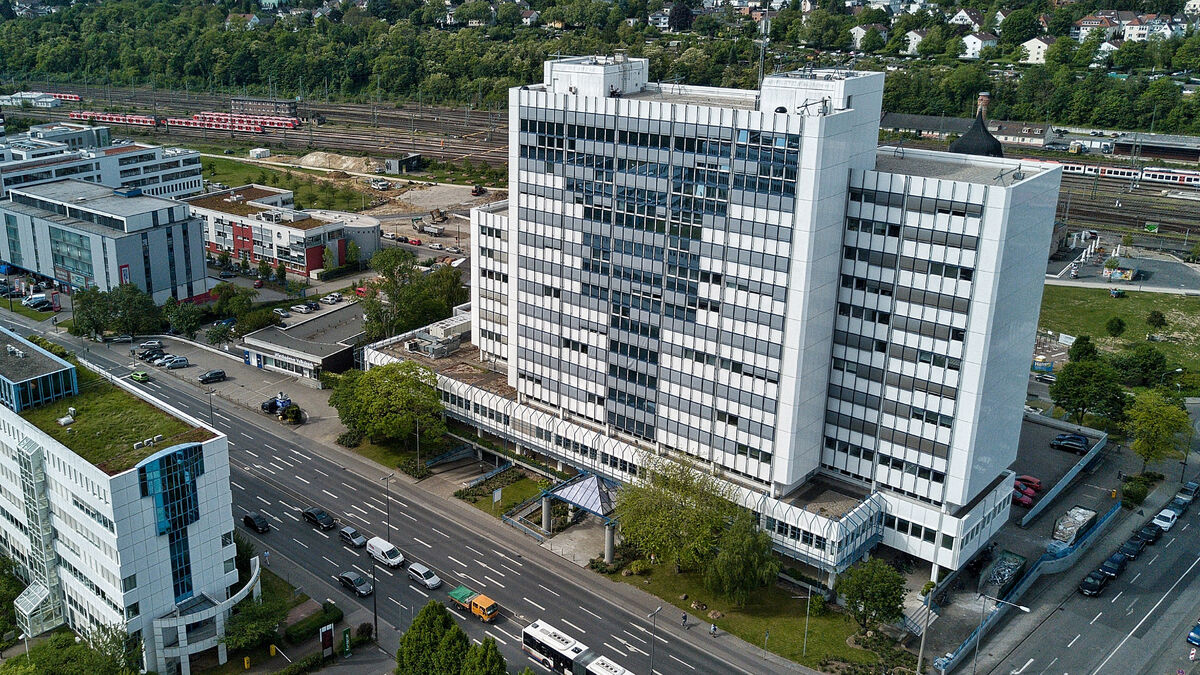
\includegraphics[width=\textwidth]{hcc.jpg}
    \caption{\acrlong{hcc}}
\end{figure}

\clearpage

\pagenumbering{Roman}

% Seitenzahl festlegen
\setcounter{page}{4}

% Literaturverzeichnis
\printbibliography[
    title=Literaturverzeichnis,
    heading=bibintoc
]

\clearpage

\pagenumbering{gobble}

\section*{Versicherung}
Ich, Max Mustermann, versichere, dass ich diese Arbeit selbstständig verfasst und keine anderen als die angegebenen Hilfsmittel benutzt habe.
Die den benutzten Hilfsmitteln wörtlich oder inhaltlich entnommenen Stellen habe ich unter Quellenangaben kenntlich gemacht.
Die Arbeit hat in gleicher oder ähnlicher Form noch keiner anderen Prüfungsbehörde vorgelegen.\\[1cm]

\noindent
Musterstadt, 15.02.2022
\end{document}